\section{前\hspace{1em}言}

语言学习作为一项复杂而多维的认知活动,长期以来一直是教育学、心理学和语言学领域的研究热点。传统的语言学习模式通常依赖于课堂、教材和教师指导,然而,随着学习理论的不断发展,越来越多的研究表明,学习环境对语言习得的效率有着深远的影响。近年来,一种新兴的语言学习模式逐渐引起学界关注——即在非传统学习环境中,通过身心放松与沉浸式体验相结合的方式,提升语言能力。本文正是基于这一背景,探讨“外语学习”与“卧榻之地”的跨界融合,试图为语言学习领域提供一种全新的视角与实践路径。

“卧榻之地”作为一种特殊的物理空间,不仅是人们日常休息与放松的场所,更因其独特的环境属性而具备了潜在的学习功能。本文提出,在“卧榻之地”中进行外语学习,不仅能够有效缓解学习者的心理压力,还能通过环境与心理的互动,增强语言记忆与应用能力。这种学习模式的提出,既是对传统语言学习方法的补充,也是对学习环境理论的进一步拓展。

本文首先从理论层面分析“卧榻之地”作为学习环境的独特优势,随后结合实践案例,探讨其在语言习得中的实际效果。最后,本文将对这种跨界融合的协同效应进行总结,并提出未来研究的方向与建议。通过本研究,我们希望能够为语言学习者提供一种更加轻松、高效的学习方式,同时也为相关领域的理论研究与实践探索提供新的思路。

如\ref{fig:learn_english}所示,作者本人在“卧榻之地”中进行外语学习的实践场景,生动展示了非传统学习环境对语言习得的潜在影响。通过这种沉浸式体验,学习者能够在身心放松的状态下,更高效地掌握语言技能。

\begin{figure}[htbp]
	\centering
	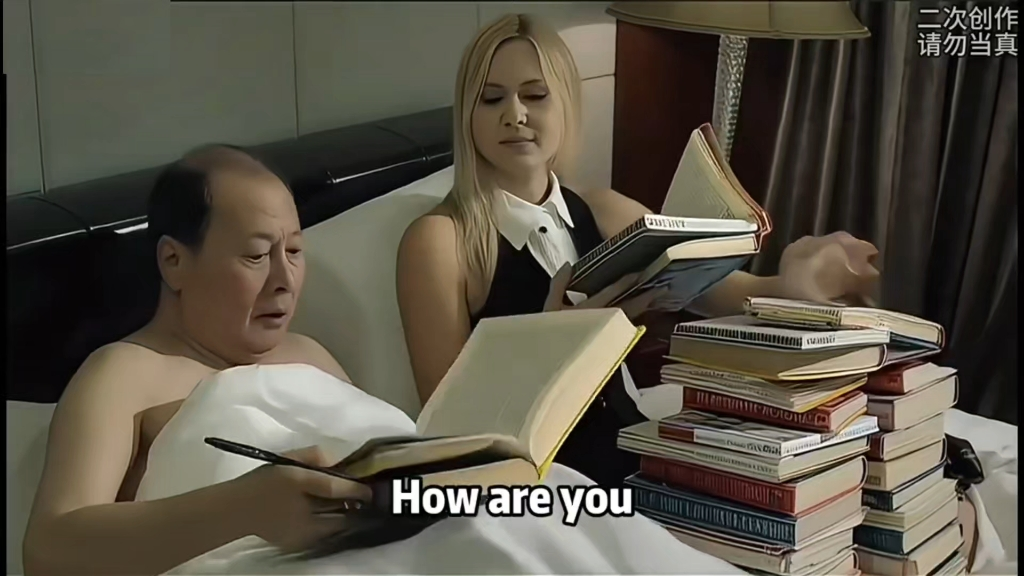
\includegraphics[width=0.8\textwidth]{./imgs/外语学习证明.jpg} % 图片路径
	\caption{作者本人“外语学习”实践场景:卧榻之地与语言习得的跨界融合\ 图源\cite{A橘色的海2025(补)假如陈清泉真的在学外语}} % 图片标题
	\label{fig:learn_english} % 图片标签
\end{figure}